%!TEX root = ../../00main.tex

\section{Kubernetes}
Kubernetes è una piattaforma portatile, estensibile e open-source per la gestione e l'orchestrazione di applicativi Cloud-Native.
La piattaforma è scritta in linguaggio Go ed è stato inizialmente sviluppato da Google per migliorare la gestione dei propri applicativi. Il progetto è attualmente parte della Cloud Native Computing Foundation\footnote{Cloud Native Computing Foundation - \url{link}}, organizzazione che promuove e mantiene progetti open-source volti all'approccio Cloud Native.
Kubernetes utilizza un insieme di oggetti fruibili tramite API per descrivere lo stato desiderato del cluster, indicando, ad esempio, quali applicazioni eseguire, quali immagini utilizzare, il numero di repliche da istanziare, quali risorse di rete e di spazio su disco rendere disponibili. L'interazione viene resa possibile grazie a kube-apiserver, il server HTTP che implementa l'API Kubernetes. L'utente ha dunque due possibilità per manipolare le configurazioni del cluster, la prima è quella di eseguire esplicitamente richieste di tipo RESTful al server API, la seconda e' quella di utilizzare kubectl, un'interfaccia da linea di comando costituita da una serie di comandi e sotto-comandi che astraggono le chiamate API.
\subsection{Architettura}
Un cluster Kubernetes è un insieme di macchine, chiamate nodi, che eseguono carichi applicativi. Il cluster deve avere almeno un Worker Node ed un Master Node. Il Worker Node è un tipo di nodo che ospita i Pod, particolari componenti di Kubernetes che contengono uno o piú container. Il Master Node è il nodo su cui viene eseguito il Control Plane, una componente fondamentale di Kubernetes che svolge le attivita operative del cluster.

\begin{figure}[H]
 \centering
 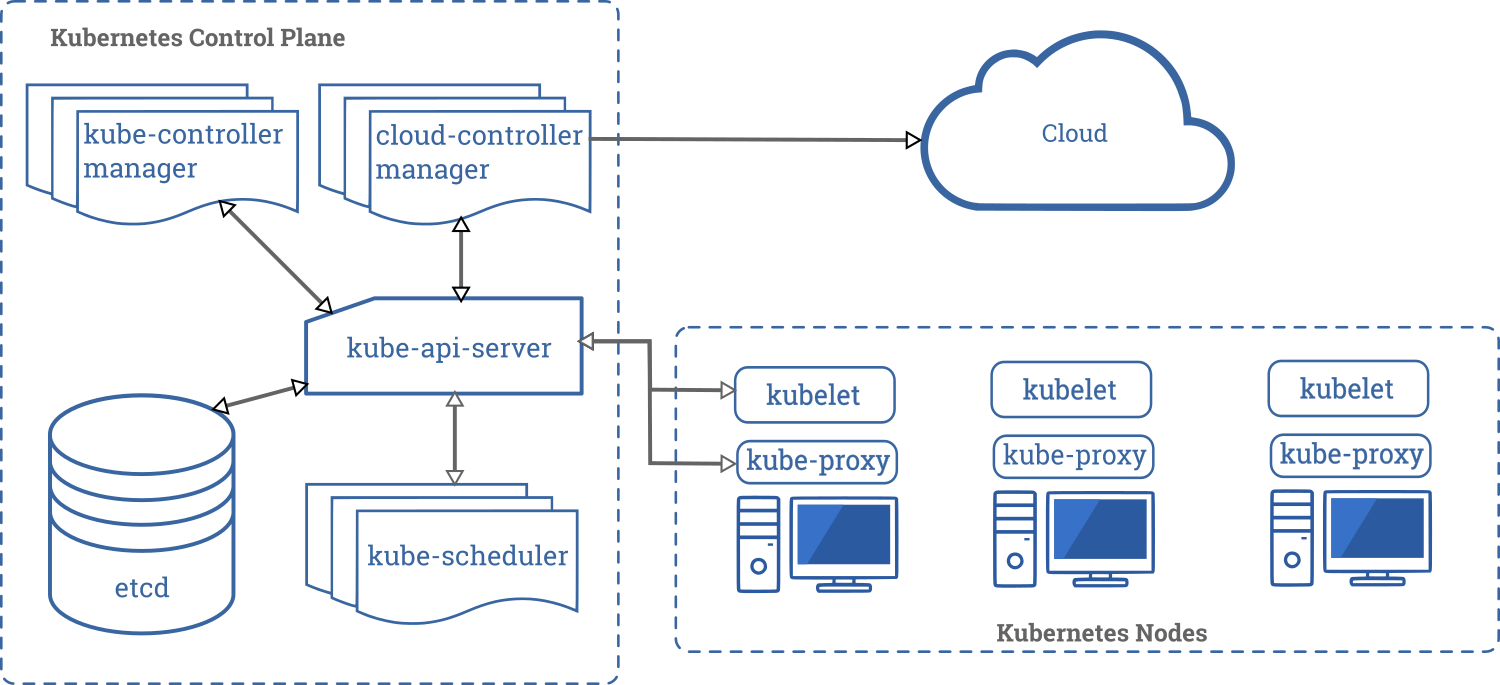
\includegraphics[width=1.0\textwidth]{./Figure/Kubernetes_Architettura.png}
 \caption{Architettura di Kubernetes}
 \label{fig:Architettura}
\end{figure}

\subsection{Componenti del Control Plane}
Il Kubernetes Control Plane è il centro nevralgico delle operazioni del cluster. È costituito da una serie di componenti, in esecuzione all'interno del cluster, che hanno il compito di garantire l'integritá esecutiva del cluster come ad esempio lo scheduling dei Worker Node e la gestione dei possibili errori dei Pod.
\begin{itemize}
    \item\textbf{kube-apiserver}
    kube-apiserver è il server API per il cluster Kubernetes. È il punto di contatto centrale a cui accedono tutti gli utenti, l'automazione e i componenti nel cluster Kubernetes. Il server API implementa un'API RESTful su HTTP, esegue tutte le operazioni API ed è responsabile dell'archiviazione degli oggetti API in un backend di archiviazione persistente.
    \item\textbf{etcd}
    etcd è la componente di archiviazione principale di Kubernetes, etcd memorizza e replica tutti gli stati dei cluster Kubernetes. Il meccanismo di memorizzazione che adotta è di tipo chiave-valore ovvero ad ogni valore memorizzato viene associato una chiave che rappresenta il suo identificatore univoco. In questo modo il Control Plane è in grado di storicizzare gli stati del Cluster confrontando lo stato attuale con quello desiderato in modo di intervenire tempestivamente in caso di necessità.
    \item\textbf{kube-scheduler}
    kube-scheduler è la componente che consente al Control Plane lo scheduling dei Pod sui nodi. il kube-scheduler controlla i pod appena creati che non hanno un nodo assegnato, e dopo averlo identificato glielo assegna. 
\end{itemize}
\subsection{Componenti del Worker Node}
Il Worker Node è il nodo del cluster su cui viene eseguito effettivamente l'applicazione. Su ogni nodo di tipo Worker Node vengono eseguiti tre componenti di Kubernetes.
\begin{itemize}
    \item{kubelet}
    La componente kubelet è un agente che è sempre in esecuzione su ogni Worker Node e ha come compito quello di controllare il ciclo di vita dei container all'interno dei Pod. La kubelet riceve un set di specifiche definite in fase di deployment dall'utente e si assicura che i container rispettino tali specifiche.
    \item{kube-proxy}
    La componente kube-proxy è un proxy eseguito su ogni Nodo, ossia un particolare componente che consente di identificare i nodi all'interno della rete del cluster e permette che essi possano comunicare sia all'interno che all'esterno del cluster.
    \item{Container Runtime} il Container Runtime è il software responsabile dell'esecuzione dei container. Kubernetes supporta tutte le implementazioni di Kubernetes CRI (Container Runtime Interface) come ad esempio Docker e containerd.
\end{itemize}
\subsection{Oggetti Kubernetes}
Kubernetes offre una varietà di oggetti per definire le specifiche del proprio sistema. Questi oggetti costituiscono entità persistenti per rappresentare lo stato del cluster, quali applicazioni sono in esecuzione e su quali nodi, le risorse da allocare e le politiche da adottare. Per istanziare un oggetto con le direttive e le informazioni desiderate, si utilizza spesso un file di tipo YAML oppure JSON.
Ciascun oggetto è caratterizzato da due campi che ne descrivono la configurazione: \\\\
\textbf{Specifiche} Le specifiche descrivono lo stato desiderato dell'oggetto, cioè le caratteristiche che deve assumere. \\\\
\textbf{Stato} Lo stato descrive lo stato attuale dell'oggetto e viene automaticamente aggiornato da Kubernetes.
\begin{itemize}
    \item\textbf{Pod}
    Un Pod costituisce la più semplice, piccola e basilare unità di esecuzione in Kubernetes. La sua natura funzionale è quella di incapsulare uno o più container e di condividerne le risorse come l'archiviazione dei dati e le risorse di rete.
    I Pod generalmente non vengono creati direttamente in Kubernetes perchè questi sono considerati oggetti effimeri. Solitamente i Pod vengono creati e gestiti da controller di più alto livello come Deployment, StatefulSet o DaemonSet.
    \item\textbf{Deployment}
    L'oggetto Deployment si occupa di creare e gestire il ciclo di vita di uno o più Pod e dei ReplicaSet.
    Un Deployment fornisce un approccio dichiarativo per la creazione e la modifica di Pod e ReplicaSet, con esso è possibile dunque descrivere lo stato che il Pod deve assumere ed il Deployment Controller si occuperà di aggiornare lo stato attuale con quello desiderato.
    \item\textbf{ReplicaSet}
    Un ReplicaSet ha il compito specifico di mantenere attive una o più copie di un Pod. Questo meccanismo garantisce la piena disponibilità del Pod a cui il ReplicaSet è agganciato in quanto nel momento in cui un Pod, per un qualsiasi motivo, cessa il suo funzionamento, verrà sostituito da una sua esatta copia.
    \item\textbf{Service}
    I Pod in Kubernetes sono entità effimere, essi vengono creati e distrutti in base allo stato desiderato del cluster. Per natura quindi non hanno un'identificazione statica all'interno della rete del cluster ma ad ogni Pod viene assegnato un indirizzo IP dinamico che varia nel tempo.
    Un Service in Kubernetes costituisce un'astrazione che definisce un insieme logico di Pod e una politica con cui accedervi.
    Kubernetes offre diversi tipi di Service:
        \subitem\textbf{ClusterIP} Espone il Service con un indirizzo IP interno al cluster, rendendo il cluster raggiungibile solo dall'interno del cluster stesso.
        \subitem\textbf{NodePort} Espone il Service su ciascun indirizzo IP corrispondente ad un nodo del cluster, su una porta scelta automaticamente, uguale per tutti i nodi.
        \subitem\textbf{LoadBalancer} Permette di esporre le applicazioni all'esterno del cluster.
    \item\textbf{Job}
    Un oggetto di tipo Job permette di eseguire e gestire task complessi all'interno del cluster. Un Job infatti permette di eseguire un insieme di Pod in maniera sequenziale o parallela considerandoli come un'unica attività di lavoro da portare a termine. Il Job terrà in esecuzione l'attività fino a quando un numero specifico di Pod non verrà terminato correttamente. Quando viene raggiunto un numero specifico di completamenti riusciti, l'attività risulterà completata ed il Job cesserà la sua esecuzione. L'eliminazione del Job distruggerà dunque tutti i Pod precedentemente assegnati. 
\end{itemize}